\documentclass[10pt]{beamer}

%%%
% PREAMBLE FOR THIS DOC 
%%%
%https://tex.stackexchange.com/questions/68821/is-it-possible-to-create-a-latex-preamble-header
\usepackage{/Users/miw267/Repos/latex_preamble/beamer_preamble}

\usetikzlibrary{matrix}



% \album{image file}{url}{artist}{album}
\newcommand{\album}[4]{%
  \begin{minipage}[t]{0.185\textwidth}\centering
    \href{#2}{\includegraphics[width=\linewidth]{#1}}\\[0.3em]
    {\small\bfseries #3}\\{\small #4}
  \end{minipage}}
  
\newcommand{\albumtiny}[4]{%
  \begin{minipage}[t]{0.185\textwidth}\centering
    \href{#2}{\includegraphics[width=\linewidth]{#1}}\\[0.3em]
    {\tiny \bfseries #3}\\{\tiny #4}
  \end{minipage}}
  
  
%%%
% DOCUMENT
%%%

\begin{document}

%\maketitle

%% Title page frame
%\begin{frame}
%    \titlepage 
%\end{frame}





\title{10/02/2026: Midterm Review Part 1: Proofs}
\author{CSCI 246: Discrete Structures}

\begin{frame}
    \titlepage 
\end{frame}


\begin{frame}

\begin{myredbox}[title=Announcements]
At beginning of class Monday, you can optionally retake any quiz of \textbf{your choice!} \\

The study guides will be the same. The questions will be different (in general).
\end{myredbox}
\vfill 


\begin{myyellowbox}[title=Today's Agenda]
\begin{itemize}
	\item Quiz (20 mins)
	\item Review of proof techniques (5-10 mins)
	\item Group exercises (20-25 mins)
%	%
%	\begin{itemize}
%	\footnotesize 
%	\item Review induction 
%	\end{itemize}
%	%
\end{itemize}

%	Rationale for group exercises: we got shortchanged on time last couple days, and I already did a lot of lectures, so I want you to practice. Next problems quiz will cover relations and functions: Hamkins and 
%	
\end{myyellowbox}
\vfill 

\end{frame}


\begin{frame}{Motivational point for this age of AI}


\small 
\colorbox{blue!30}{\textbf{Finding:}} A person's computer science skills, cognitive ability, and writing ability are strong predictors of the quality of software produced when using LLM coding agents.


\begin{center}
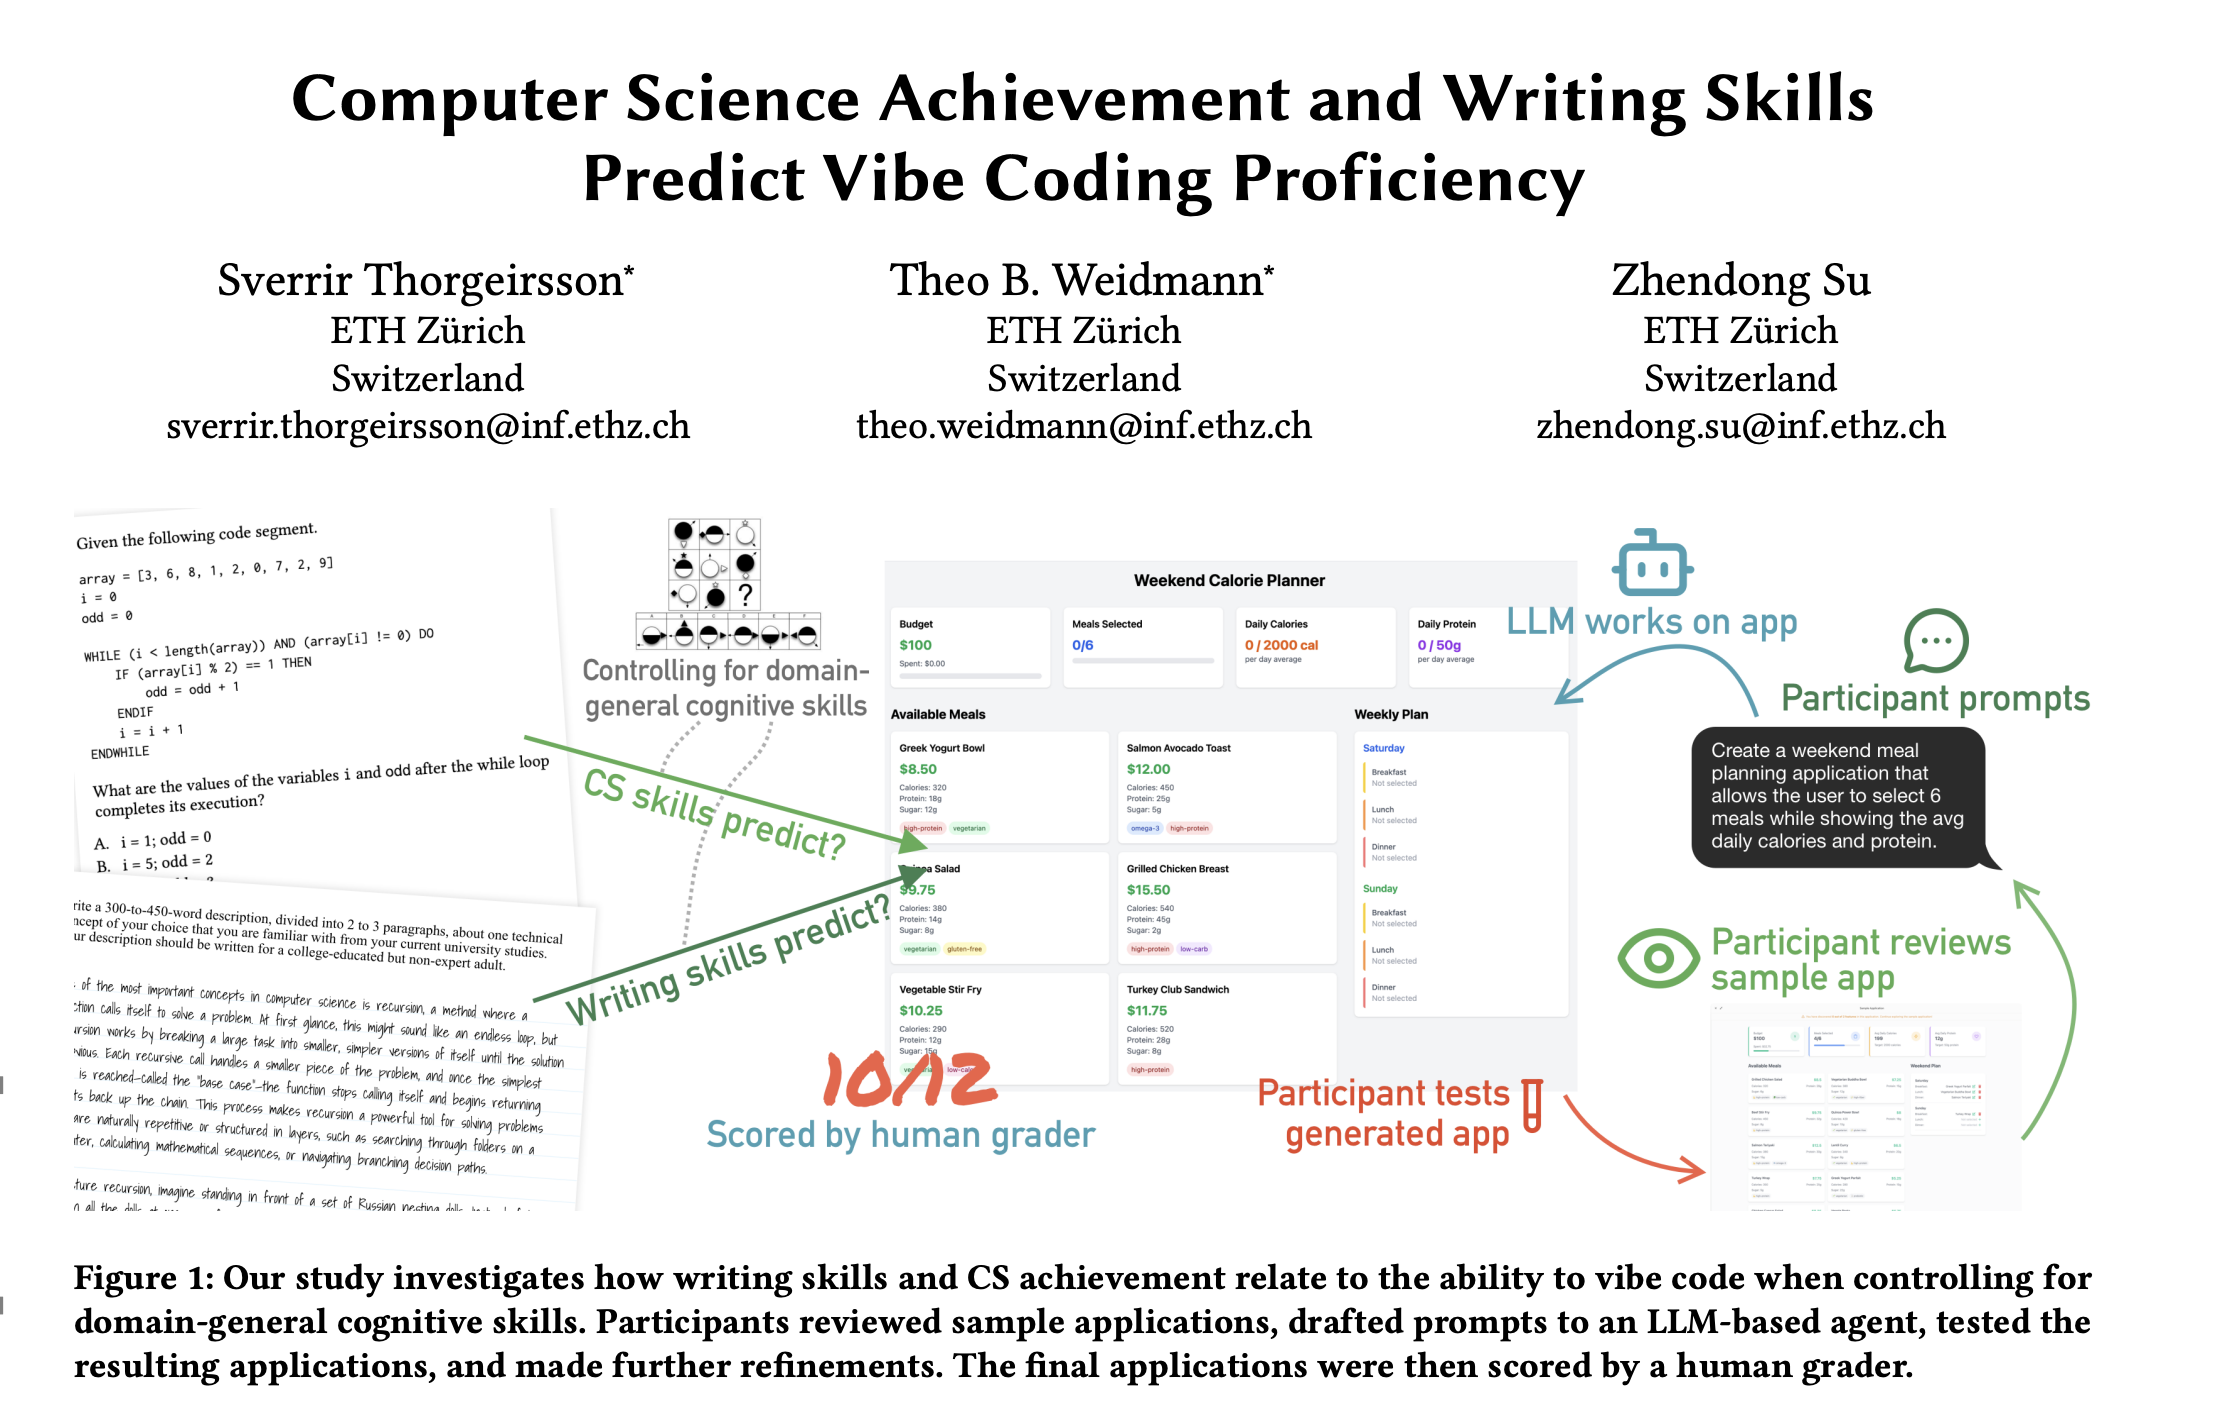
\includegraphics[width=0.8\textwidth]{images/vibe_coding.png}	
\evsrc{Thorgeirsson, Sverrir, Theo B. Weidmann, and Zhendong Su. "Computer science achievement and writing skills predict vibe coding proficiency." In Proceedings of the 2026 CHI Conference on Human Factors in Computing Systems, pp. 1-17. 2026.}
\end{center}

\end{frame}


\begin{frame}{Weekly Quiz \#5}

\begin{enumerate}
	\item (Partitions.) How many different anagrams (including nonsensical words) can be made from the word \texttt{bookkeeper}? Justify your answer.
	\item (Relations.) Consider the relation $\leq$ (less than or equal to) on the integers.  Is the relation reflexive? Symmetric? Transitive? Justify your answers.
	\item (Equivalence relations.) Let $n$ be a positive integer.  Prove that congruence modulo $n$ is an equivalence relation on the set of integers.
\end{enumerate}
\vfill
\begin{mygreenbox}[title=\text{Reference Material: Definition}]
Let $n$ be a positive integer.  We say that integers $x$ and $y$ are \textbf{congruent modulo n}, and we write 
\[x \equiv y \quad \text{(mod $n$)} \]
if $n | (x-y)$.
\end{mygreenbox}

	
\end{frame}


\begin{frame}[standout]
Review of proofs
\end{frame}

\begin{frame}

\begin{mybluebox}[title=Proof Template: Direct proof of an if-then (if $A$ then $B$) theorem]

\begin{enumerate}
	\item Write down the if-then statement you're trying to prove. 
	\item At the beginning of the proof, write down the \textit{antecedent} (the A in  \texttt{if A then B}) as your assumption. 
	\item  At the end of the proof, write down the \textit{consequent} (the B in  \texttt{if A then B}) as your conclusion. 
	\item Unravel the definitions, working forward from the beginning of the proof and backward from the end of the proof.
	\item Forge a link between the two halves of the argument.
\end{enumerate}
\end{mybluebox}
\evsrc{\hfill Scheinerman Proof Template 1}
	
\end{frame}


\begin{frame}{Example}
\textbf{Proposition.} The square of an odd integer is odd.

\textbf{Proof.}

\begin{tabularx}{\textwidth}{|L{3cm}|X|}
\hline \textbf{Annotation} & \textbf{Main Text} \\ \hline
 \hlorange{Convert Prop. to ``if-then" form} &  \hlorange{We show that if $x$ is an odd integer, then $x^2$ is odd.} \\ \hline
\hlblue{State antecedent} & \hlblue{Let $x$ be an odd integer.} \\ \hline
\hlgreen{Unravel defs.} & \hlgreen{Then by definition of \textit{odd}, there is an integer $a$ such that $x=2a+1$.} \\ \hline
\hlred{*** The glue ***} &   \hlred{So $x^2= (2a+1)(2a+1) = 4a^2+4a+1 = 2 (2a^2+2a) +1$.} \\ \hline
 \hlgreen{Unravel defs.} & \hlgreen{So there is an integer $b$ \red{(where $b=2a^2+2a$)} such that $x^2=2b+1$.} \\ \hline
  \hlblue{State consequent} & \hlblue{Hence, $x^2$ is odd.} \\ \hline
\hline
\end{tabularx}
\end{frame}



\begin{frame}

\begin{mybluebox}[title=Proof Template: Direct proof of an if-and-only-if theorem]

To prove a statement of the form \qq{A iff B}:
\begin{itemize}
\item ($\implies$) Prove \qq{If A, then B}.
\item ($\impliedby$) Prove \qq{If B, then A}.
\end{itemize}
\end{mybluebox}
\evsrc{\hfill Scheinerman Proof Template 2}
\end{frame}


\begin{frame}

\begin{mybluebox}[title=Proof Template: Refuting a false if-then statement via a counterexample]

To disprove a statement of the form \qq{If A then B}: \\
\hspace*{1.5em}  Find an instance where $A$ is true but $B$ is false.
	
\end{mybluebox}
\evsrc{\hfill Scheinerman Proof Template 3}

\vfill
\pause 
\colorbox{red!30}{\textbf{Note.}} Often, you'll need to \alert{justify} that $A$ is true (by showing that the conditions of the relevant definition is satisfied.)
\end{frame}


\begin{frame}

\begin{mybluebox}[title=Proof Template: Proving one set is a subset of another]
To show $A \subseteq B$: \\
\hspace*{1.5em} Show that if $x \in A$, then $x \in B$.
\end{mybluebox}
\evsrc{\hfill Scheinerman Proof Template 6}

\end{frame}


\begin{frame}

\begin{mybluebox}[title=Proof Template: Proving two sets are equal]
Let $A$ and $B$ be sets.  To show $A = B$: 
\begin{itemize}
	\item Show $A \subseteq B$.
	\item Show $B \subseteq A$.
\end{itemize}
\end{mybluebox}
\evsrc{\hfill Scheinerman Proof Template 6}
\vfill
\pause
\colorbox{blue!30}{\textbf{Remark.}} In other words, we must show:
\begin{itemize}
	\item If $x \in A$, then $x \in B$.
	\item If $x \in B$, then $x \in A$.
\end{itemize}

\end{frame}

\begin{frame}[standout]
Group exercises
\end{frame}

\begin{frame}
\begin{columns}
\begin{column}{0.33\textwidth}
Ashley, Isabelle: 7 \\ 
Bailey, Tanna: 7 \\ 
Blaisdell, Olyver: 5 \\ 
Brown, Ashton: 1 \\ 
Brown, Jonathan: 2 \\ 
Cardenas, Dominic: 2 \\ 
Cutler, George: 11 \\ 
Fabik, Roland: 8 \\ 
Fellows, Audrey: 10 \\ 
Fitzgerald, Ryan: 8 \\ 
Fuller, Ryan: 6 \\ 
Griffen, Clara: 4 \\ 
Grutsch, Tanner: 12 \\\end{column}
\begin{column}{0.33\textwidth}
Hager, Nathan: 11 \\ 
Horner, Jayden: 7 \\ 
Johnson, Jaret: 3 \\ 
Kintzel, Samantha: 1 \\ 
Lameres, Alexis: 9 \\ 
Lee, Holden: 5 \\ 
Mayala, Reece: 6 \\ 
McLean, Connor: 12 \\ 
Mcbride, Daniel: 10 \\ 
Miller, Maverick: 2 \\ 
Moss, Emily: 8 \\ 
Mousseau, Matthew: 3 \\ 
Neuman, Evan: 13 \\\end{column}
\begin{column}{0.33\textwidth}
Putnam, John: 5 \\ 
Ramos, Vydel: 10 \\ 
Rathbun, Jedidiah: 9 \\ 
Roberts, Matthew: 13 \\ 
Roller, Nathan: 4 \\ 
Ryan, Otis: 3 \\ 
Shevtsov, Timothy: 1 \\ 
Sinclair, Aidan: 11 \\ 
Smith, Charles: 6 \\ 
Stensland, Emma: 13 \\ 
Thiessen, Logan: 9 \\ 
Thompson, Jaiden: 4 \\ 
Vath, Ethan: 12 \\\end{column}
\end{columns}
\end{frame}


\begin{frame}{Group exercises}
\begin{enumerate}
	\item  Prove that the product of two even integers is even.
	\item  Let $x$ be an integer. Prove that $0 \mid x$ if and only if $x=0$.
	\item Disprove: If $p$ and $q$ are prime, then $p+q$ is composite.
	\item Let $A = \set{x \in \mathbb{Z} : 4 \mid x}$ and let $B = \set{x \in \mathbb{Z} : 2 \mid x}$. Show that $A \subseteq B$. 
	\item Let $A = \set{n \in \mathbb{Z} : 3 \mid n}$ and let $B = \set{n \in \mathbb{Z} : 3 \mid (n+6)}$. Show that $A=B$. 
\end{enumerate}
\vfill
\small 
\begin{mygreenbox}[title={Reference: Definitions}]
\begin{itemize}
	\item Let $a,b$ be integers.  We say that $a$ is \textbf{divisible} by $b$, written $b \mid a$, if there is an integer $c$ such that $bc=a$. We call $b$ a \textbf{divisor} of $a$.
	\item An integer is called \textbf{even} if it is divisible by 2. (That is, an integer $x$ is even if there is an integer $c$ such that $x=2c$.)
	\item An integer $p$ is called \textbf{prime} if $p>1$ and the only positive divisors of $p$ are 1 and $p$.
	\item A positive integer $a$ is called \textbf{composite} if there is an integer $b$ such that  $1<b<a$ and $b \mid a$.
\end{itemize}
	
\end{mygreenbox}

\end{frame}


\end{document}
